\section{Appendix}

\subsection{Ensemble Learning Methods}
\label{appendix:ensemble}

Three ensemble models in total was investigated in this study: Weighted Average, Bagging and AdaBoost. 

As the name suggests, weighted average produces the final prediction by taking the weighted mean of the predictions from the base models, using the performance as measured by the Spearman correlation between the predicted and observed on-target activity as the weight. 

Bagging is a method that trains multiple models on different subsets of the training data, hoping to 

AdaBoost is a boosting ensemble method that trains multiple models sequentially. 

\begin{figure}[h]
    \centering
    \begin{subfigure}{0.4\textwidth}
        \centering
        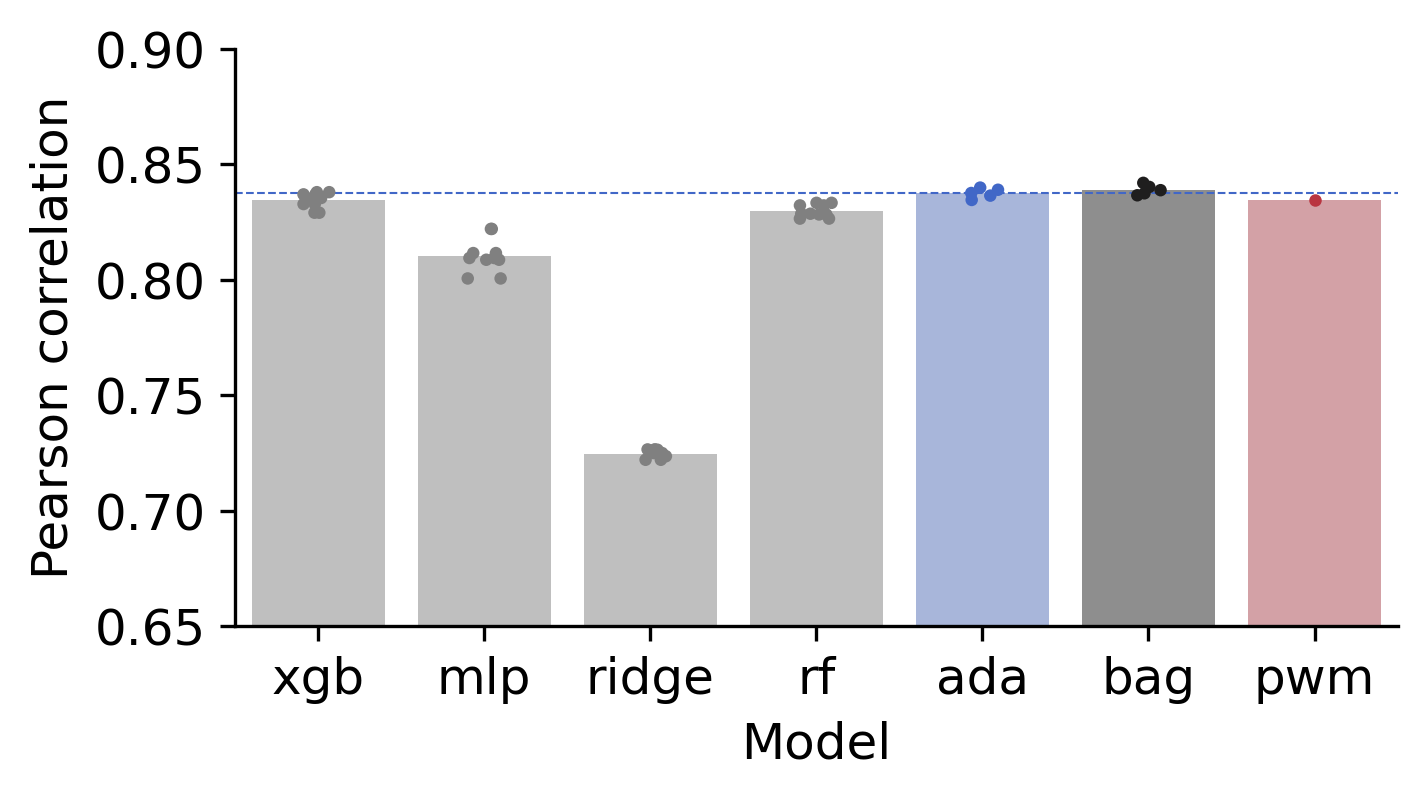
\includegraphics[width=\linewidth]{ensemble_comparison_Pearson.png}
        \caption{Pearson correlation}
    \end{subfigure}
    \begin{subfigure}{0.4\textwidth}
        \centering
        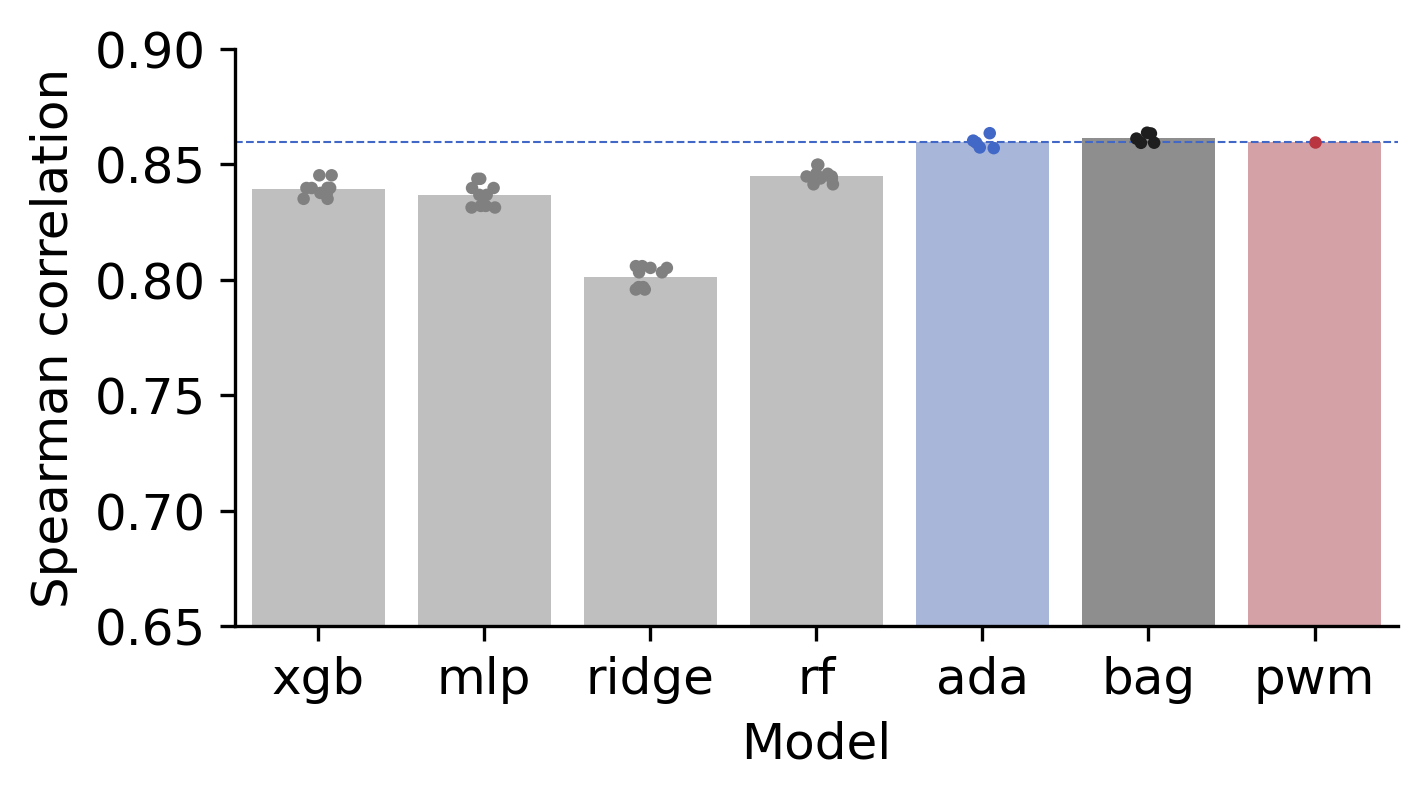
\includegraphics[width=\linewidth]{ensemble_comparison_Spearman.png}
        \caption{Spearman correlation}
    \end{subfigure}
    \caption{Comparison of ensemble learning methods' performance using (a) Pearson correlation and (b) Spearman correlation.}
    \label{fig:ensemble_comparison}
\end{figure}


\subsection{Features used by DeepPrime, PRIDICT 1.0/2.0 and conventional ML methods}

